\section{Controllable generation}
The continuous structure of our framework allows us to not only produce data samples from $p_0$, but also from $p_0(\bfx(0) \mid \bfy)$ if $p_t(\bfy \mid \bfx(t))$ is known. %
Given a forward SDE as in \cref{eqn:forward_sde}, we can sample from $p_t(\bfx(t) \mid \bfy)$ by starting from $p_T(\bfx(T) \mid \bfy)$ and solving a conditional reverse-time SDE:
\begin{align}
\ud \bfx = \{\bff(\bfx, t) - g(t)^2[ \nabla_\bfx  \log p_t(\bfx)+  \nabla_{\bfx}  \log p_t(\bfy \mid \bfx)]\} \ud t + g(t) \ud \bar{\bfw}.\label{eqn:cond_sde}
\end{align}
In general, we can use \cref{eqn:cond_sde} to solve a large family of \emph{inverse problems} with score-based generative models, once given an estimate of the gradient of the forward process, $\nabla_\bfx \log p_t(\bfy \mid \bfx(t) )$. In some cases, it is possible to train a separate model to learn the forward process $\log p_t(\bfy \mid \bfx(t))$ and compute its gradient. Otherwise, we may estimate the gradient with heuristics and domain knowledge. In \cref{app:inverse_prob}, we provide a broadly applicable method for obtaining such an estimate without the need of training auxiliary models.

We consider three applications of controllable generation with this approach: class-conditional generation, image imputation and colorization. When $\bfy$ represents class labels, we can train a time-dependent classifier $p_t(\bfy \mid \bfx(t))$ for class-conditional sampling. Since the forward SDE is tractable, we can easily create training data $(\bfx(t), \bfy)$ for the time-dependent classifier
by first sampling $(\bfx(0), \bfy)$ from a dataset, and then sampling $\bfx(t) \sim p_{0t}(\bfx(t) \mid \bfx(0))$. Afterwards, we may employ a mixture of cross-entropy losses over different time steps, like \cref{eqn:training}, to train the time-dependent classifier $p_t(\bfy \mid \bfx(t))$. We provide class-conditional CIFAR-10 samples in \cref{fig:cond_gen} (left), and relegate more details and results to \cref{app:cond_gen}.

Imputation is a special case of conditional sampling.
Suppose we have an incomplete data point $\bfy$ where only some subset, $\Omega(\bfy)$ is known. Imputation amounts to sampling from $p(\bfx(0) \mid \Omega(\bfy))$, which we can accomplish using an unconditional model (see \cref{app:imputation}). Colorization is a special case of imputation, except that the known data dimensions are coupled. We can decouple these data dimensions with an orthogonal linear transformation, and perform imputation in the transformed space (details in \cref{app:colorization}). \cref{fig:cond_gen} (right) shows results for inpainting and colorization achieved with unconditional time-dependent score-based models.


\begin{figure}
    \centering
    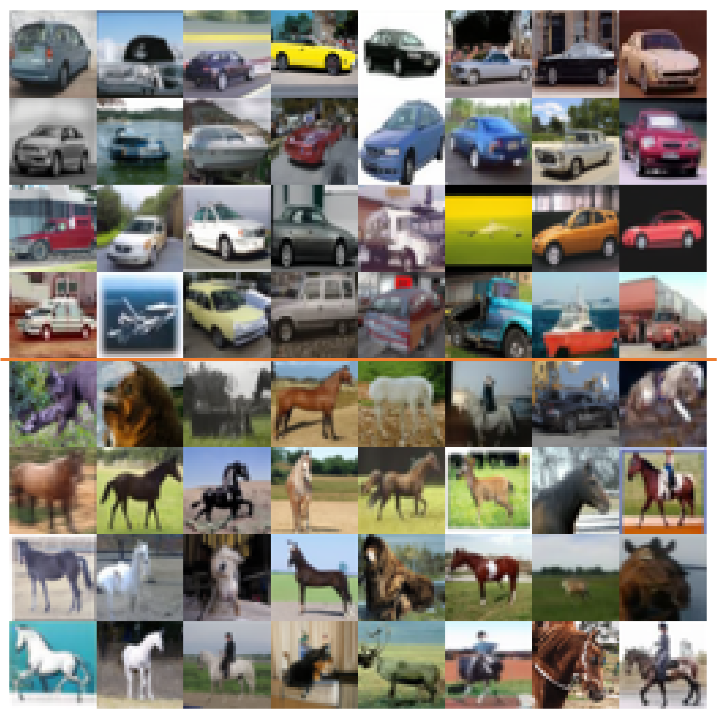
\includegraphics[width=0.327\linewidth, trim=5 0 7 0, clip, valign=c]{figures/cond_gen_line.png}
    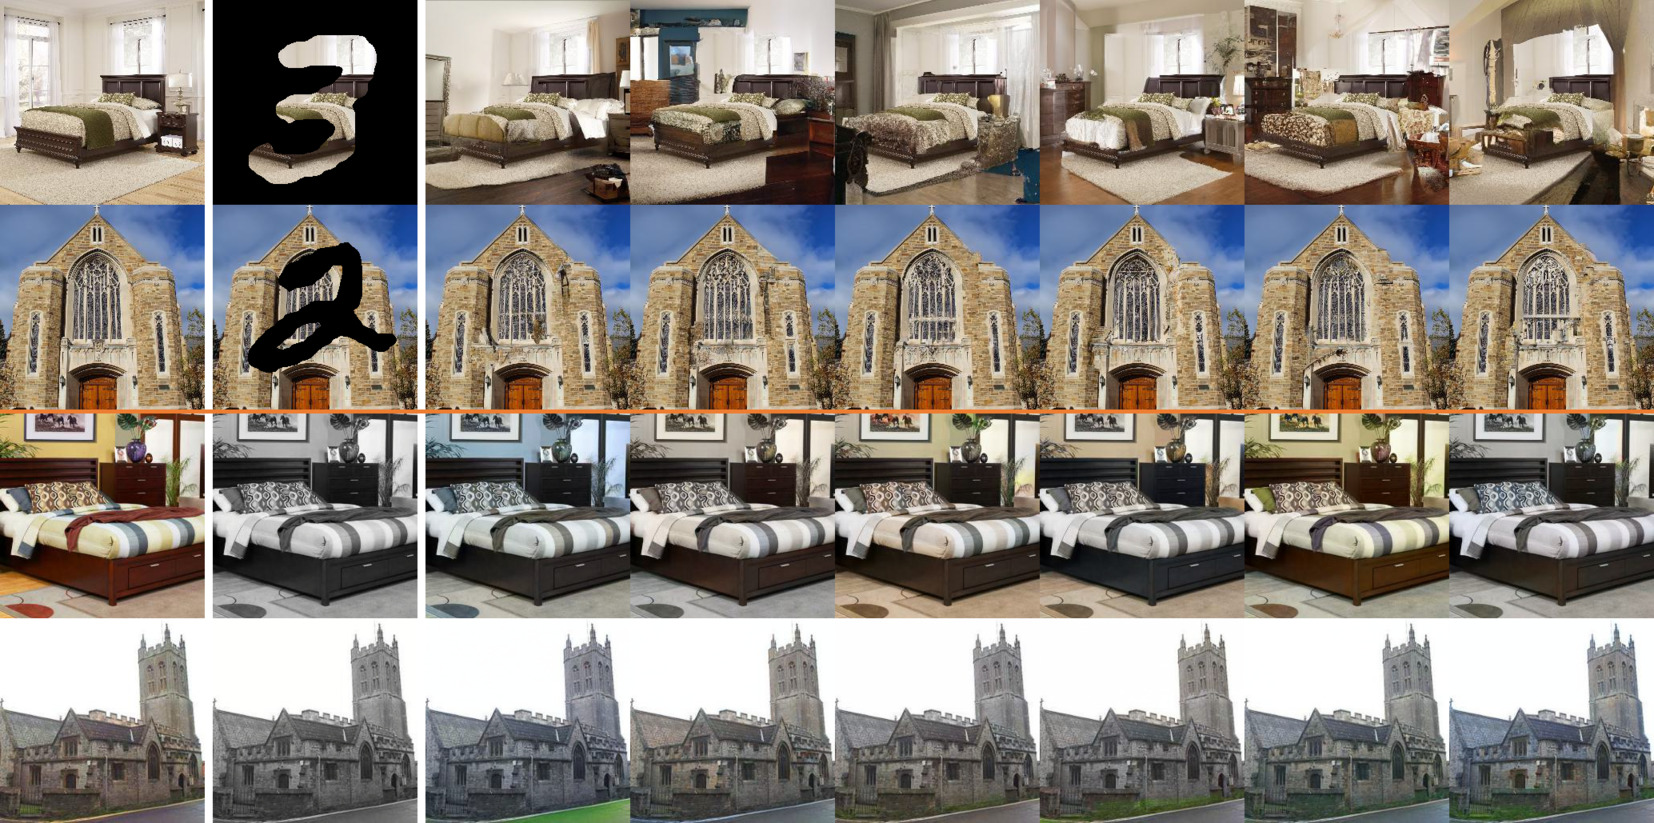
\includegraphics[width=0.66\linewidth, valign=c]{figures/inpaint_colorization.jpg}
    \caption{\textit{Left}: Class-conditional samples on $32\times 32$ CIFAR-10. Top four rows are automobiles and bottom four rows are horses. \textit{Right:} Inpainting (top two rows) and colorization (bottom two rows) results on $256\times 256$ LSUN. First column is the original image, second column is the masked/gray-scale image, remaining columns are sampled image completions or colorizations.}
    \label{fig:cond_gen}
\end{figure}
